\documentclass[]{book}
\usepackage{lmodern}
\usepackage{amssymb,amsmath}
\usepackage{ifxetex,ifluatex}
\usepackage{fixltx2e} % provides \textsubscript
\ifnum 0\ifxetex 1\fi\ifluatex 1\fi=0 % if pdftex
  \usepackage[T1]{fontenc}
  \usepackage[utf8]{inputenc}
\else % if luatex or xelatex
  \ifxetex
    \usepackage{mathspec}
  \else
    \usepackage{fontspec}
  \fi
  \defaultfontfeatures{Ligatures=TeX,Scale=MatchLowercase}
\fi
% use upquote if available, for straight quotes in verbatim environments
\IfFileExists{upquote.sty}{\usepackage{upquote}}{}
% use microtype if available
\IfFileExists{microtype.sty}{%
\usepackage{microtype}
\UseMicrotypeSet[protrusion]{basicmath} % disable protrusion for tt fonts
}{}
\usepackage[margin=1in]{geometry}
\usepackage{hyperref}
\hypersetup{unicode=true,
            pdftitle={Решение упражнений из книги R Science},
            pdfauthor={Stas Masuta},
            pdfborder={0 0 0},
            breaklinks=true}
\urlstyle{same}  % don't use monospace font for urls
\usepackage{natbib}
\bibliographystyle{apalike}
\usepackage{color}
\usepackage{fancyvrb}
\newcommand{\VerbBar}{|}
\newcommand{\VERB}{\Verb[commandchars=\\\{\}]}
\DefineVerbatimEnvironment{Highlighting}{Verbatim}{commandchars=\\\{\}}
% Add ',fontsize=\small' for more characters per line
\usepackage{framed}
\definecolor{shadecolor}{RGB}{248,248,248}
\newenvironment{Shaded}{\begin{snugshade}}{\end{snugshade}}
\newcommand{\KeywordTok}[1]{\textcolor[rgb]{0.13,0.29,0.53}{\textbf{#1}}}
\newcommand{\DataTypeTok}[1]{\textcolor[rgb]{0.13,0.29,0.53}{#1}}
\newcommand{\DecValTok}[1]{\textcolor[rgb]{0.00,0.00,0.81}{#1}}
\newcommand{\BaseNTok}[1]{\textcolor[rgb]{0.00,0.00,0.81}{#1}}
\newcommand{\FloatTok}[1]{\textcolor[rgb]{0.00,0.00,0.81}{#1}}
\newcommand{\ConstantTok}[1]{\textcolor[rgb]{0.00,0.00,0.00}{#1}}
\newcommand{\CharTok}[1]{\textcolor[rgb]{0.31,0.60,0.02}{#1}}
\newcommand{\SpecialCharTok}[1]{\textcolor[rgb]{0.00,0.00,0.00}{#1}}
\newcommand{\StringTok}[1]{\textcolor[rgb]{0.31,0.60,0.02}{#1}}
\newcommand{\VerbatimStringTok}[1]{\textcolor[rgb]{0.31,0.60,0.02}{#1}}
\newcommand{\SpecialStringTok}[1]{\textcolor[rgb]{0.31,0.60,0.02}{#1}}
\newcommand{\ImportTok}[1]{#1}
\newcommand{\CommentTok}[1]{\textcolor[rgb]{0.56,0.35,0.01}{\textit{#1}}}
\newcommand{\DocumentationTok}[1]{\textcolor[rgb]{0.56,0.35,0.01}{\textbf{\textit{#1}}}}
\newcommand{\AnnotationTok}[1]{\textcolor[rgb]{0.56,0.35,0.01}{\textbf{\textit{#1}}}}
\newcommand{\CommentVarTok}[1]{\textcolor[rgb]{0.56,0.35,0.01}{\textbf{\textit{#1}}}}
\newcommand{\OtherTok}[1]{\textcolor[rgb]{0.56,0.35,0.01}{#1}}
\newcommand{\FunctionTok}[1]{\textcolor[rgb]{0.00,0.00,0.00}{#1}}
\newcommand{\VariableTok}[1]{\textcolor[rgb]{0.00,0.00,0.00}{#1}}
\newcommand{\ControlFlowTok}[1]{\textcolor[rgb]{0.13,0.29,0.53}{\textbf{#1}}}
\newcommand{\OperatorTok}[1]{\textcolor[rgb]{0.81,0.36,0.00}{\textbf{#1}}}
\newcommand{\BuiltInTok}[1]{#1}
\newcommand{\ExtensionTok}[1]{#1}
\newcommand{\PreprocessorTok}[1]{\textcolor[rgb]{0.56,0.35,0.01}{\textit{#1}}}
\newcommand{\AttributeTok}[1]{\textcolor[rgb]{0.77,0.63,0.00}{#1}}
\newcommand{\RegionMarkerTok}[1]{#1}
\newcommand{\InformationTok}[1]{\textcolor[rgb]{0.56,0.35,0.01}{\textbf{\textit{#1}}}}
\newcommand{\WarningTok}[1]{\textcolor[rgb]{0.56,0.35,0.01}{\textbf{\textit{#1}}}}
\newcommand{\AlertTok}[1]{\textcolor[rgb]{0.94,0.16,0.16}{#1}}
\newcommand{\ErrorTok}[1]{\textcolor[rgb]{0.64,0.00,0.00}{\textbf{#1}}}
\newcommand{\NormalTok}[1]{#1}
\usepackage{longtable,booktabs}
\usepackage{graphicx,grffile}
\makeatletter
\def\maxwidth{\ifdim\Gin@nat@width>\linewidth\linewidth\else\Gin@nat@width\fi}
\def\maxheight{\ifdim\Gin@nat@height>\textheight\textheight\else\Gin@nat@height\fi}
\makeatother
% Scale images if necessary, so that they will not overflow the page
% margins by default, and it is still possible to overwrite the defaults
% using explicit options in \includegraphics[width, height, ...]{}
\setkeys{Gin}{width=\maxwidth,height=\maxheight,keepaspectratio}
\IfFileExists{parskip.sty}{%
\usepackage{parskip}
}{% else
\setlength{\parindent}{0pt}
\setlength{\parskip}{6pt plus 2pt minus 1pt}
}
\setlength{\emergencystretch}{3em}  % prevent overfull lines
\providecommand{\tightlist}{%
  \setlength{\itemsep}{0pt}\setlength{\parskip}{0pt}}
\setcounter{secnumdepth}{5}
% Redefines (sub)paragraphs to behave more like sections
\ifx\paragraph\undefined\else
\let\oldparagraph\paragraph
\renewcommand{\paragraph}[1]{\oldparagraph{#1}\mbox{}}
\fi
\ifx\subparagraph\undefined\else
\let\oldsubparagraph\subparagraph
\renewcommand{\subparagraph}[1]{\oldsubparagraph{#1}\mbox{}}
\fi

%%% Use protect on footnotes to avoid problems with footnotes in titles
\let\rmarkdownfootnote\footnote%
\def\footnote{\protect\rmarkdownfootnote}

%%% Change title format to be more compact
\usepackage{titling}

% Create subtitle command for use in maketitle
\newcommand{\subtitle}[1]{
  \posttitle{
    \begin{center}\large#1\end{center}
    }
}

\setlength{\droptitle}{-2em}

  \title{Решение упражнений из книги R Science}
    \pretitle{\vspace{\droptitle}\centering\huge}
  \posttitle{\par}
    \author{Stas Masuta}
    \preauthor{\centering\large\emph}
  \postauthor{\par}
      \predate{\centering\large\emph}
  \postdate{\par}
    \date{2018-09-03}

\usepackage{booktabs}

\begin{document}
\maketitle

{
\setcounter{tocdepth}{1}
\tableofcontents
}
\chapter{Введение}

Это электронная версия решений упражнений, свёрстанная при помощи
\textbf{bookdown}, который можно установить здесь:

\begin{Shaded}
\begin{Highlighting}[]
\KeywordTok{install.packages}\NormalTok{(}\StringTok{"bookdown"}\NormalTok{)}
\CommentTok{# or the development version}
\CommentTok{# devtools::install_github("rstudio/bookdown")}
\end{Highlighting}
\end{Shaded}

\chapter{Introduction}\label{introduction}

\section*{Acknowledgments}\label{acknowledgments}
\addcontentsline{toc}{section}{Acknowledgments}

All the credit should go to Garrett Grolemund and Hadley Wickham for
writing the truly fantastic \emph{R for Data Science} book, without
which these solutions would not exist---literally.

\chapter{Предварительный анализ}\label{-}

\section{Введение}\label{-1}

Электронная версия книги по адресу \url{http://r4ds.had.co.nz}.

Для начала работы подключаем библиотеку

\begin{Shaded}
\begin{Highlighting}[]
\KeywordTok{library}\NormalTok{(}\StringTok{"tidyverse"}\NormalTok{)}
\end{Highlighting}
\end{Shaded}

Не было упражнений.

\section{Первые шаги}\label{-}

\subsection*{Упражнение 3.2.1}\label{-3.2.1}
\addcontentsline{toc}{subsection}{Упражнение 3.2.1}

Run \texttt{ggplot(data\ =\ mpg)} what do you see? \{.unnumbered\}

\begin{Shaded}
\begin{Highlighting}[]
\KeywordTok{ggplot}\NormalTok{(}\DataTypeTok{data =}\NormalTok{ mpg)}
\end{Highlighting}
\end{Shaded}


\includegraphics{homework_files/figure-latex/unnamed-chunk-3-1.pdf}

Пустое окно построения. Функция \texttt{ggplot()} из пакета
\texttt{ggplot2} только содаёт область построения, функциями мы
производим наполнение области построения. Больше инфы смотри в подсказке
\url{https://github.com/rstudio/cheatsheets/blob/master/data-visualization-2.1.pdf}
.

\subsection*{Упражнение 3.2.2}\label{-3.2.2}
\addcontentsline{toc}{subsection}{Упражнение 3.2.2}

How many rows are in \texttt{mpg}? How many columns? \{.unnumbered\}
Чтобы проверить ``строение'' фрейма данных \texttt{mpg},можно
воспользоваться двумя способами. Var1:

\begin{Shaded}
\begin{Highlighting}[]
\NormalTok{ggplot2}\OperatorTok{::}\NormalTok{mpg}
\end{Highlighting}
\end{Shaded}

\begin{verbatim}
## # A tibble: 234 x 11
##    manufacturer model displ  year   cyl trans drv     cty   hwy fl    cla~
##    <chr>        <chr> <dbl> <int> <int> <chr> <chr> <int> <int> <chr> <ch>
##  1 audi         a4      1.8  1999     4 auto~ f        18    29 p     com~
##  2 audi         a4      1.8  1999     4 manu~ f        21    29 p     com~
##  3 audi         a4      2    2008     4 manu~ f        20    31 p     com~
##  4 audi         a4      2    2008     4 auto~ f        21    30 p     com~
##  5 audi         a4      2.8  1999     6 auto~ f        16    26 p     com~
##  6 audi         a4      2.8  1999     6 manu~ f        18    26 p     com~
##  7 audi         a4      3.1  2008     6 auto~ f        18    27 p     com~
##  8 audi         a4 q~   1.8  1999     4 manu~ 4        18    26 p     com~
##  9 audi         a4 q~   1.8  1999     4 auto~ 4        16    25 p     com~
## 10 audi         a4 q~   2    2008     4 manu~ 4        20    28 p     com~
## # ... with 224 more rows
\end{verbatim}

где видно что \texttt{mpg} это матрица 234 строки на 11 столбцов.

Var2:

\begin{Shaded}
\begin{Highlighting}[]
\KeywordTok{glimpse}\NormalTok{(mpg)}
\end{Highlighting}
\end{Shaded}

\begin{verbatim}
## Observations: 234
## Variables: 11
## $ manufacturer <chr> "audi", "audi", "audi", "audi", "audi", "audi", "...
## $ model        <chr> "a4", "a4", "a4", "a4", "a4", "a4", "a4", "a4 qua...
## $ displ        <dbl> 1.8, 1.8, 2.0, 2.0, 2.8, 2.8, 3.1, 1.8, 1.8, 2.0,...
## $ year         <int> 1999, 1999, 2008, 2008, 1999, 1999, 2008, 1999, 1...
## $ cyl          <int> 4, 4, 4, 4, 6, 6, 6, 4, 4, 4, 4, 6, 6, 6, 6, 6, 6...
## $ trans        <chr> "auto(l5)", "manual(m5)", "manual(m6)", "auto(av)...
## $ drv          <chr> "f", "f", "f", "f", "f", "f", "f", "4", "4", "4",...
## $ cty          <int> 18, 21, 20, 21, 16, 18, 18, 18, 16, 20, 19, 15, 1...
## $ hwy          <int> 29, 29, 31, 30, 26, 26, 27, 26, 25, 28, 27, 25, 2...
## $ fl           <chr> "p", "p", "p", "p", "p", "p", "p", "p", "p", "p",...
## $ class        <chr> "compact", "compact", "compact", "compact", "comp...
\end{verbatim}

\subsection*{Упражнение 3.2.3}\label{-3.2.3}
\addcontentsline{toc}{subsection}{Упражнение 3.2.3}

What does the \texttt{drv} variable describe? Read the help for
\texttt{?mpg} to find out. \{.unnumbered\} \texttt{drv} --- это имя
одного из параметров, оно обозначает тип привода автомобиля.

\begin{longtable}[]{@{}lc@{}}
\toprule
Краткое название & Тип привода\tabularnewline
\midrule
\endhead
f & передний\tabularnewline
r & задний\tabularnewline
4 & полный\tabularnewline
\bottomrule
\end{longtable}

\subsection*{Упражнение 3.2.4}\label{-3.2.4}
\addcontentsline{toc}{subsection}{Упражнение 3.2.4}

Make a scatter plot of \texttt{hwy} vs \texttt{cyl}. \{.unnumbered\}

можно прописывать на одной координатной плоскости разные геометрические
функции с индивидуальными параметрами, тогда правильнее будет писать вот
так

Var 1

\begin{Shaded}
\begin{Highlighting}[]
\KeywordTok{ggplot}\NormalTok{(}\DataTypeTok{data =}\NormalTok{ mpg)}\OperatorTok{+}
\StringTok{  }\KeywordTok{geom_point}\NormalTok{(}\DataTypeTok{mapping =} \KeywordTok{aes}\NormalTok{(}\DataTypeTok{x =}\NormalTok{ hwy, }\DataTypeTok{y =}\NormalTok{ cyl))}
\end{Highlighting}
\end{Shaded}

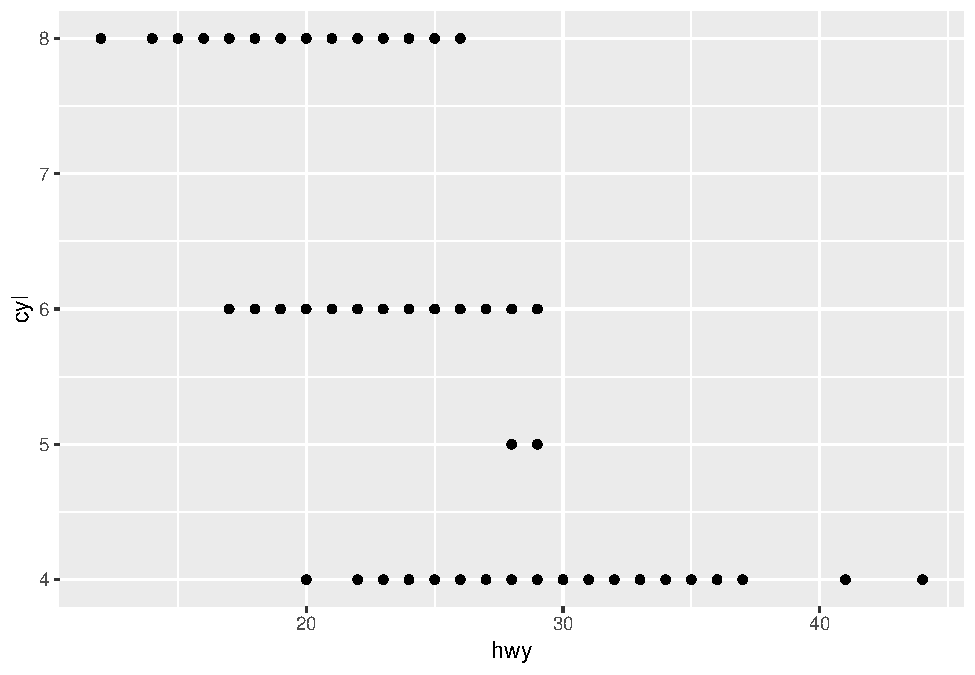
\includegraphics{homework_files/figure-latex/41-1.pdf}

Но если параметры одни и те же, а требуется построить разные геометрии,
то лучше прописать общие параметры вынося их ``за скобки'' Var 2

\begin{Shaded}
\begin{Highlighting}[]
\KeywordTok{ggplot}\NormalTok{(}\DataTypeTok{data =}\NormalTok{ mpg, }\KeywordTok{aes}\NormalTok{(}\DataTypeTok{x =}\NormalTok{ hwy, }\DataTypeTok{y =}\NormalTok{ cyl))}\OperatorTok{+}
\StringTok{ }\KeywordTok{geom_point}\NormalTok{()}
\end{Highlighting}
\end{Shaded}

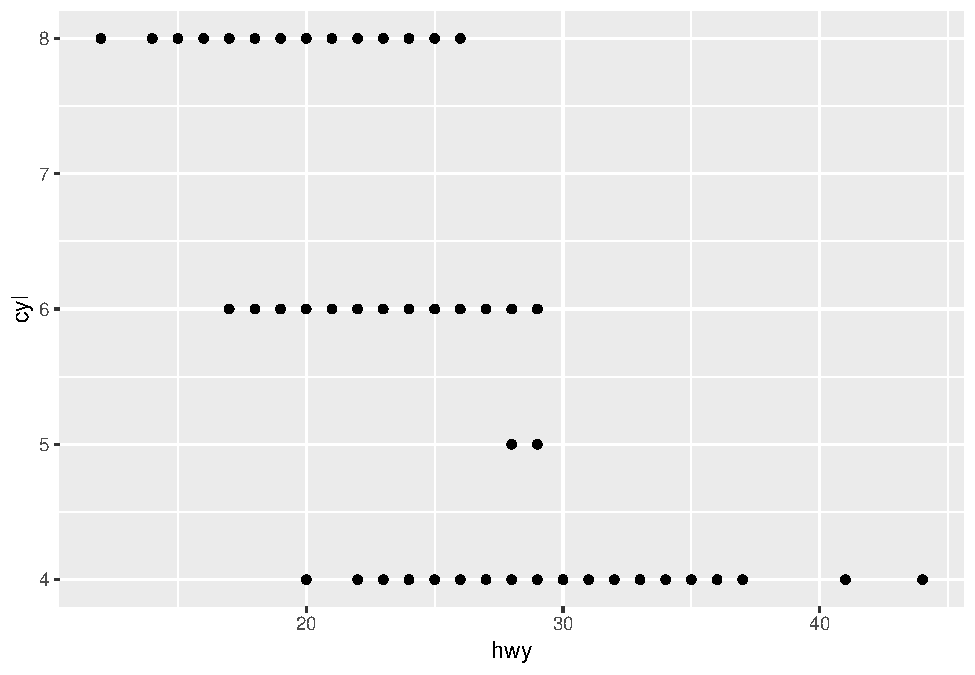
\includegraphics{homework_files/figure-latex/unnamed-chunk-6-1.pdf}

\subsection*{Упражнение 3.2.5}\label{-3.2.5}
\addcontentsline{toc}{subsection}{Упражнение 3.2.5}

What happens if you make a scatterplot of \texttt{class} vs
\texttt{drv}? Why is the plot not useful? Оба параметра являются
категориальными, или описательными. Можно построить
\texttt{\textless{}chr\textgreater{}} от
\texttt{\textless{}chr\textgreater{}}.

\begin{Shaded}
\begin{Highlighting}[]
\KeywordTok{ggplot}\NormalTok{(}\DataTypeTok{data =}\NormalTok{ mpg) }\OperatorTok{+}\StringTok{ }\KeywordTok{geom_point}\NormalTok{(}\DataTypeTok{mapping =} \KeywordTok{aes}\NormalTok{(}\DataTypeTok{x =}\NormalTok{ class, }\DataTypeTok{y =}\NormalTok{ drv))}
\end{Highlighting}
\end{Shaded}

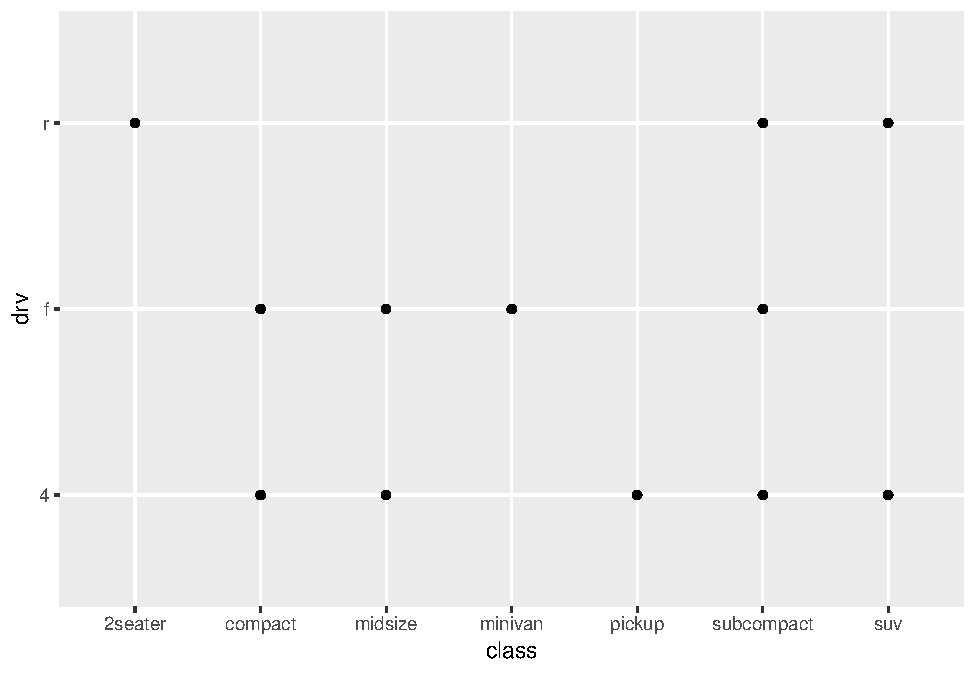
\includegraphics{homework_files/figure-latex/unnamed-chunk-7-1.pdf}

Но с точки зрения аналитики, такая информация не несёт большой пользы. В
конкретном примере можно только сказать что, все автомобили класса
2seater имеют задний привод. А в классе subcompact есть все типы
привода.

\section{Эстетика визуализации}\label{-}

\subsection*{Упражнения 3.3.1}\label{-3.3.1}
\addcontentsline{toc}{subsection}{Упражнения 3.3.1}

What's gone wrong with this code? Why are the points not blue?
\{.unnumbered\}

\begin{Shaded}
\begin{Highlighting}[]
\KeywordTok{ggplot}\NormalTok{(}\DataTypeTok{data =}\NormalTok{ mpg) }\OperatorTok{+}
\StringTok{  }\KeywordTok{geom_point}\NormalTok{(}\DataTypeTok{mapping =} \KeywordTok{aes}\NormalTok{(}\DataTypeTok{x =}\NormalTok{ displ, }\DataTypeTok{y =}\NormalTok{ hwy, }\DataTypeTok{colour =} \StringTok{"blue"}\NormalTok{))}
\end{Highlighting}
\end{Shaded}

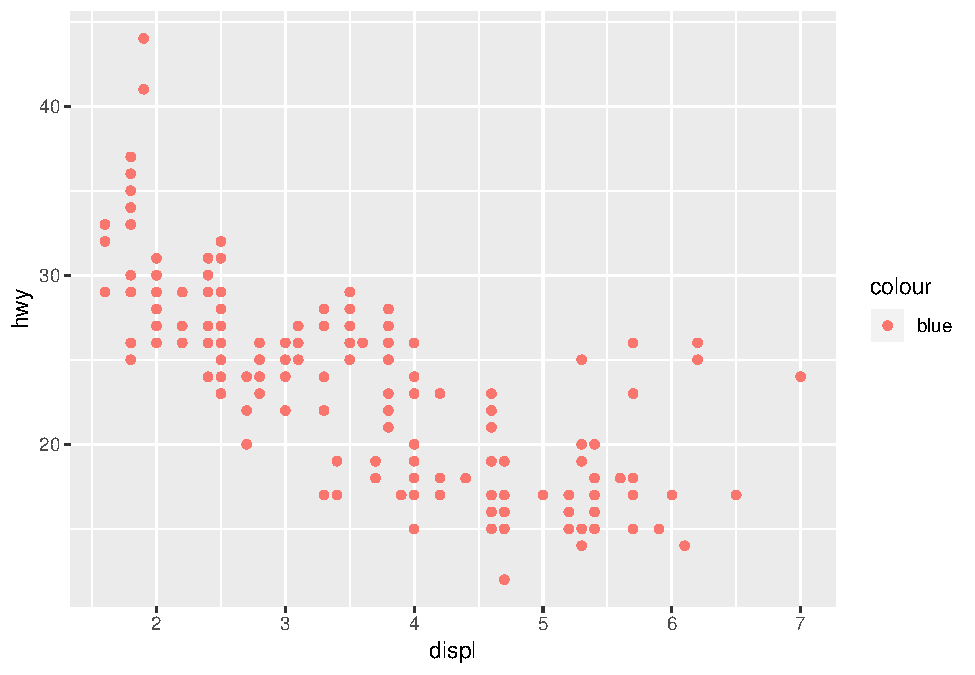
\includegraphics{homework_files/figure-latex/unnamed-chunk-8-1.pdf}

Всё потому что \texttt{colour} не вынес за скобки, потому что
\texttt{colour} это параметр функции \texttt{geom\_point()}, not
\texttt{aes()} правильно вот так

\begin{Shaded}
\begin{Highlighting}[]
\KeywordTok{ggplot}\NormalTok{(}\DataTypeTok{data =}\NormalTok{ mpg) }\OperatorTok{+}
\StringTok{  }\KeywordTok{geom_point}\NormalTok{(}\DataTypeTok{mapping =} \KeywordTok{aes}\NormalTok{(}\DataTypeTok{x =}\NormalTok{ displ, }\DataTypeTok{y =}\NormalTok{ hwy), }\DataTypeTok{colour =} \StringTok{"blue"}\NormalTok{)}
\end{Highlighting}
\end{Shaded}

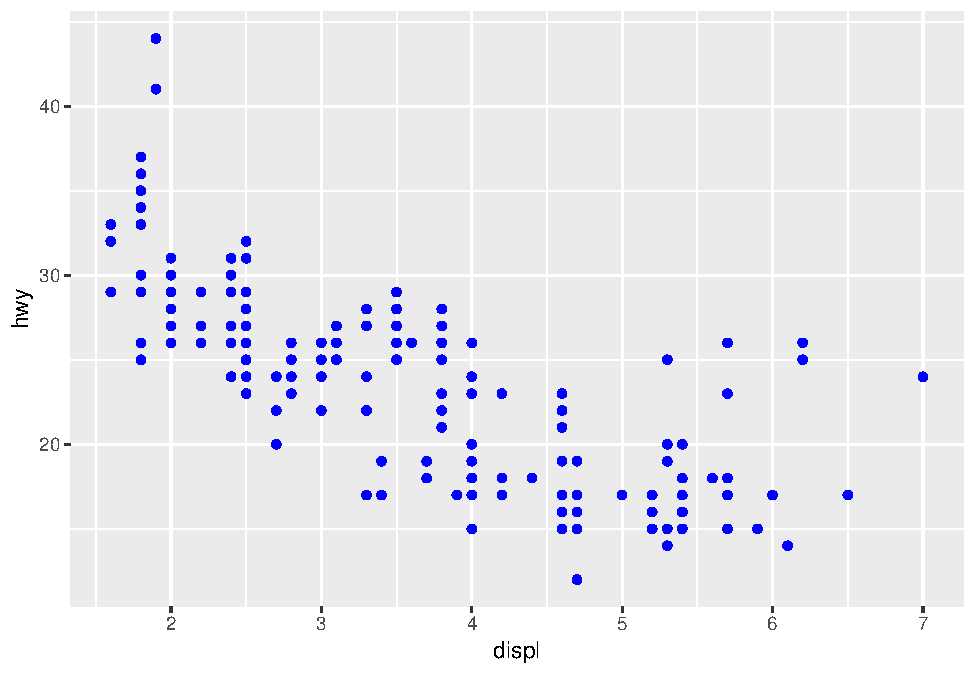
\includegraphics{homework_files/figure-latex/unnamed-chunk-9-1.pdf}

\subsection*{Упражнения 3.3.2}\label{-3.3.2}
\addcontentsline{toc}{subsection}{Упражнения 3.3.2}

Which variables in \texttt{mpg} are categorical? Which variables are
continuous? (Hint: type \texttt{?mpg} to read the documentation for the
dataset). How can you see this information when you run \texttt{mpg}?
\{.unnumbered\}

Это те факторы, которые позволяют разделить на показатели. Чтобы понять
какие факторы являются категориальными можно воспользоваться функцией
\texttt{glimpse()}, которая показывает тип каждого столбца.
Соответственно, те что \texttt{\textless{}chr\textgreater{}} и есть
категориальные:

\begin{Shaded}
\begin{Highlighting}[]
\KeywordTok{glimpse}\NormalTok{(mpg)}
\end{Highlighting}
\end{Shaded}

\begin{verbatim}
## Observations: 234
## Variables: 11
## $ manufacturer <chr> "audi", "audi", "audi", "audi", "audi", "audi", "...
## $ model        <chr> "a4", "a4", "a4", "a4", "a4", "a4", "a4", "a4 qua...
## $ displ        <dbl> 1.8, 1.8, 2.0, 2.0, 2.8, 2.8, 3.1, 1.8, 1.8, 2.0,...
## $ year         <int> 1999, 1999, 2008, 2008, 1999, 1999, 2008, 1999, 1...
## $ cyl          <int> 4, 4, 4, 4, 6, 6, 6, 4, 4, 4, 4, 6, 6, 6, 6, 6, 6...
## $ trans        <chr> "auto(l5)", "manual(m5)", "manual(m6)", "auto(av)...
## $ drv          <chr> "f", "f", "f", "f", "f", "f", "f", "4", "4", "4",...
## $ cty          <int> 18, 21, 20, 21, 16, 18, 18, 18, 16, 20, 19, 15, 1...
## $ hwy          <int> 29, 29, 31, 30, 26, 26, 27, 26, 25, 28, 27, 25, 2...
## $ fl           <chr> "p", "p", "p", "p", "p", "p", "p", "p", "p", "p",...
## $ class        <chr> "compact", "compact", "compact", "compact", "comp...
\end{verbatim}

\subsection*{Упражнения 3.3.3}\label{-3.3.3}
\addcontentsline{toc}{subsection}{Упражнения 3.3.3}

Map a continuous variable to \texttt{color}, \texttt{size}, and
\texttt{shape}. How do these aesthetics behave differently for
categorical vs.~continuous variables? \{.unnumbered\} Непрерывные
переменные, это такие переменные которые принимают значения в некотором
диапазоне. Непрерывной переменной является например \texttt{cty}, city
miles per gallon, и показывает сколько проедет автомобиль в черте горда
на один галлон топлива. Если сопоставить этой переменной \textbf{цвет}
то получится

\begin{Shaded}
\begin{Highlighting}[]
\KeywordTok{ggplot}\NormalTok{(mpg, }\KeywordTok{aes}\NormalTok{(}\DataTypeTok{x =}\NormalTok{ displ, }\DataTypeTok{y =}\NormalTok{ hwy, }\DataTypeTok{colour =}\NormalTok{ cty)) }\OperatorTok{+}
\StringTok{   }\KeywordTok{geom_point}\NormalTok{()}
\end{Highlighting}
\end{Shaded}

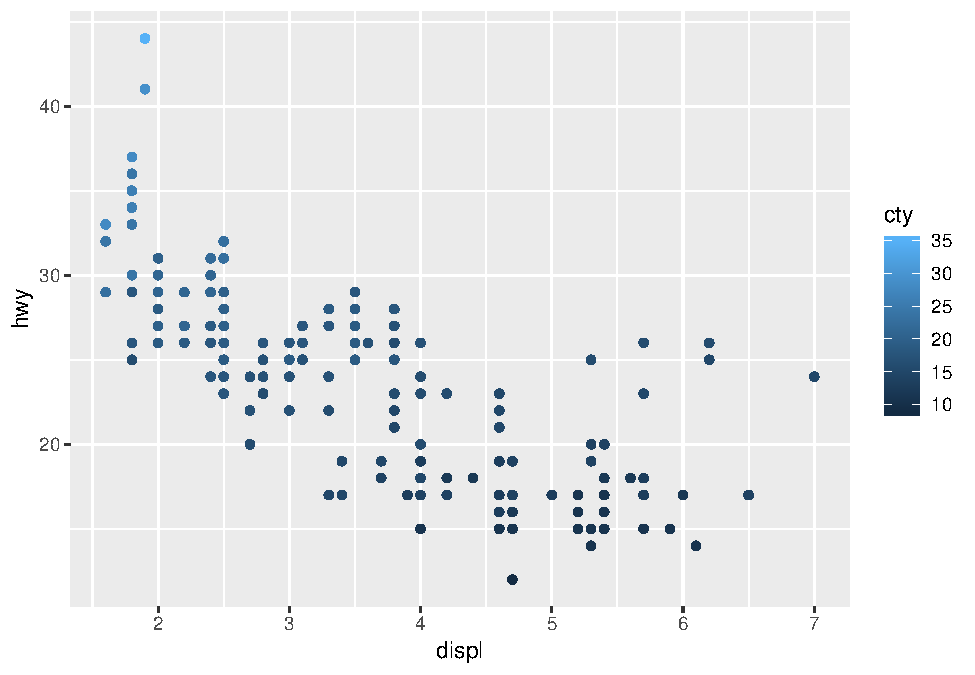
\includegraphics{homework_files/figure-latex/unnamed-chunk-11-1.pdf}

Цвет распределяется в диапазоне переменной \texttt{cty}, то есть в
пределах от примерно 10 до 35. Попробуем теперь соспоставить
\textbf{размер}

\begin{Shaded}
\begin{Highlighting}[]
\KeywordTok{ggplot}\NormalTok{(mpg, }\KeywordTok{aes}\NormalTok{(}\DataTypeTok{x =}\NormalTok{ displ, }\DataTypeTok{y =}\NormalTok{ hwy, }\DataTypeTok{size =}\NormalTok{ cty)) }\OperatorTok{+}
\StringTok{   }\KeywordTok{geom_point}\NormalTok{()}
\end{Highlighting}
\end{Shaded}

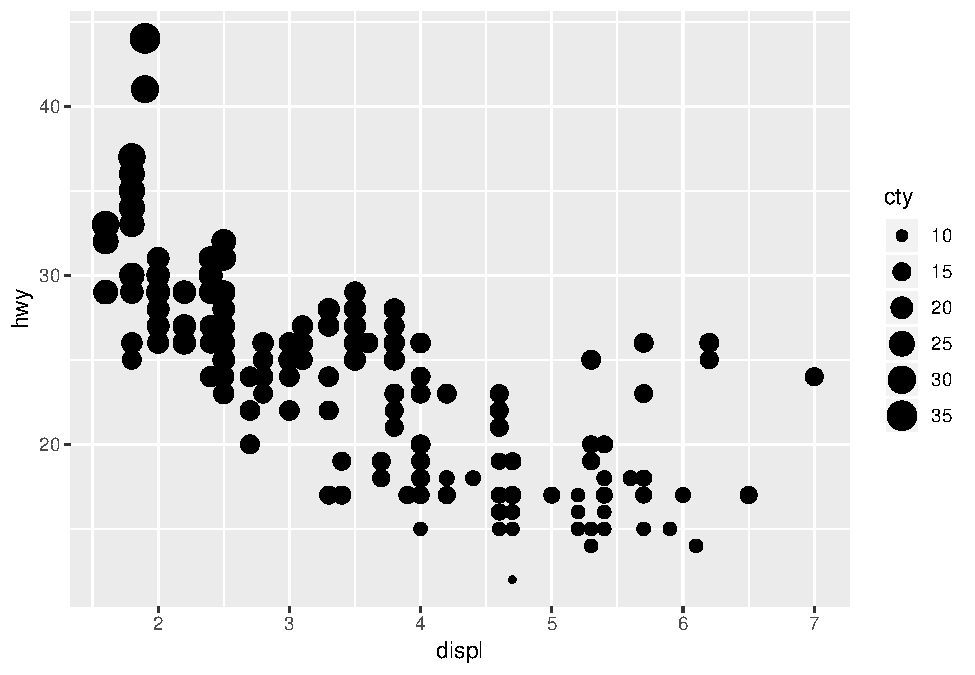
\includegraphics{homework_files/figure-latex/unnamed-chunk-12-1.pdf}

В принципе получается такая же картина, только точки выделены не цветом,
а размером. И наконец, сопоставим \textbf{форму} непрерывной переменной

\begin{Shaded}
\begin{Highlighting}[]
\CommentTok{#ggplot(mpg, aes(x = displ, y = hwy, shape = cty)) + geom_point()}
\end{Highlighting}
\end{Shaded}

А вот хуюшки. Программа выдаст
\texttt{Ошибка:\ A\ continuous\ variable\ can\ not\ be\ mapped\ to\ shape}.
Непрерывные переменные не соотносятся с атрибутом \texttt{shape}, так
сделано специально. Потому что фигур всего 24, а наборов значений у
непрерывной переменной может быть сколь угодно много

\subsection*{Упражнения 3.3.4}\label{-3.3.4}
\addcontentsline{toc}{subsection}{Упражнения 3.3.4}

What happens if you map the same variable to multiple aesthetics?
\{.unnumbered\} Связать можно, вот например, переменная \texttt{drv} для
цвета и для формы

\begin{Shaded}
\begin{Highlighting}[]
\KeywordTok{ggplot}\NormalTok{(mpg, }\KeywordTok{aes}\NormalTok{(}\DataTypeTok{x =}\NormalTok{ displ, }\DataTypeTok{y =}\NormalTok{ hwy, }\DataTypeTok{color =}\NormalTok{ drv, }\DataTypeTok{shape =}\NormalTok{ drv)) }\OperatorTok{+}\StringTok{ }\KeywordTok{geom_point}\NormalTok{()}
\end{Highlighting}
\end{Shaded}

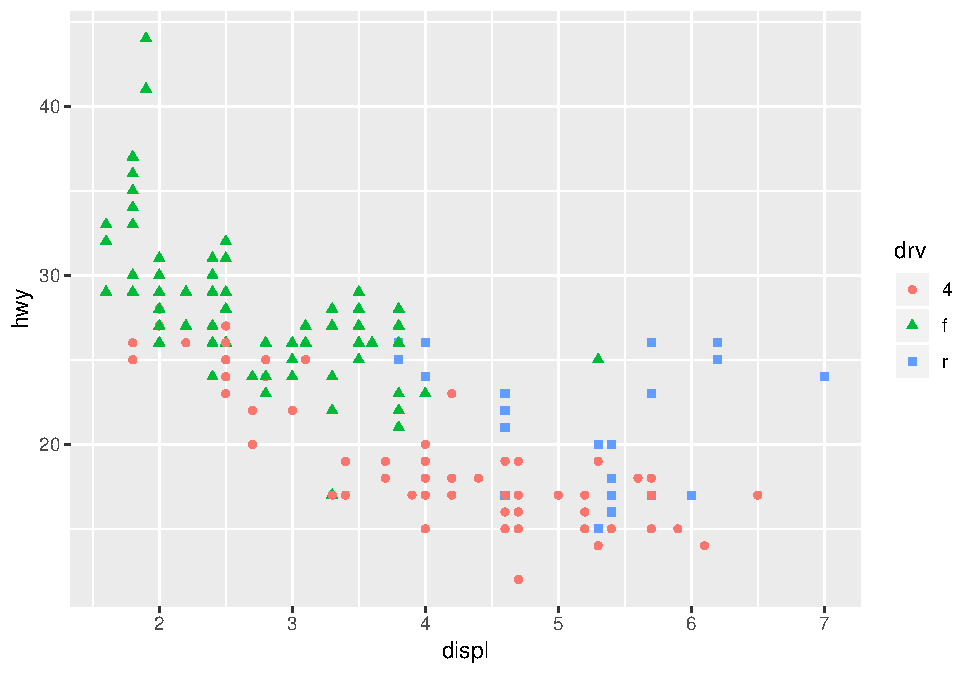
\includegraphics{homework_files/figure-latex/unnamed-chunk-14-1.pdf}

но это будет избыточное выделение.

\subsection*{Упражнения 3.3.5}\label{-3.3.5}
\addcontentsline{toc}{subsection}{Упражнения 3.3.5}

What does the \texttt{stroke} aesthetic do? What shapes does it work
with? (Hint: use \texttt{?geom\_point})

\texttt{stroke} это размер границы фигуры. Он работает с фигурами, у
которых помимо полной заливки есть цвет границы т.е. фигуры 21-24
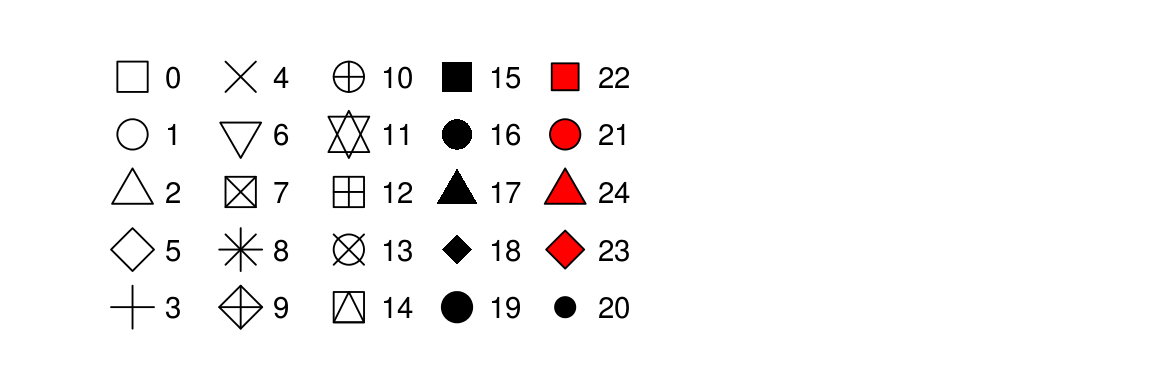
\includegraphics{img/shapes.png}

Иллюстрирующий пример. Вот построение обычными точками

\begin{Shaded}
\begin{Highlighting}[]
\KeywordTok{ggplot}\NormalTok{(mpg, }\KeywordTok{aes}\NormalTok{(hwy, cyl))}\OperatorTok{+}
\StringTok{ }\KeywordTok{geom_point}\NormalTok{()}
\end{Highlighting}
\end{Shaded}

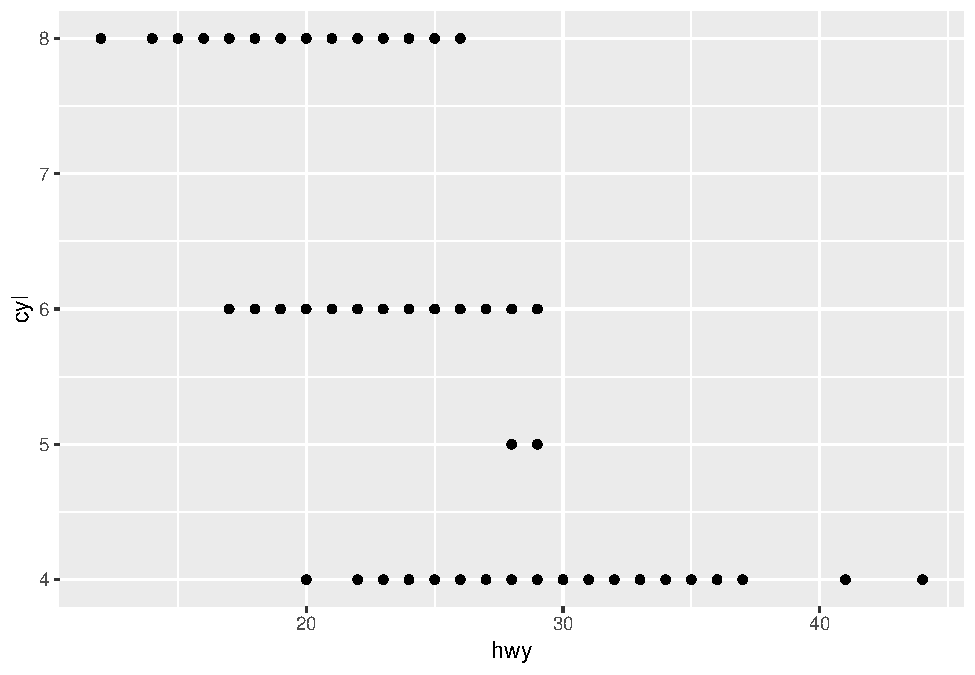
\includegraphics{homework_files/figure-latex/unnamed-chunk-15-1.pdf}

Теперь зададим красную заливку, и размер границы фигуры \(2\)

\begin{Shaded}
\begin{Highlighting}[]
\KeywordTok{ggplot}\NormalTok{(mpg, }\KeywordTok{aes}\NormalTok{(hwy, cyl)) }\OperatorTok{+}
\StringTok{ }\KeywordTok{geom_point}\NormalTok{(}\DataTypeTok{shape=}\DecValTok{21}\NormalTok{,}\DataTypeTok{colour=}\StringTok{"black"}\NormalTok{,}\DataTypeTok{fill=}\StringTok{"red"}\NormalTok{,}\DataTypeTok{size=}\DecValTok{3}\NormalTok{,}\DataTypeTok{stroke=}\DecValTok{2}\NormalTok{)}
\end{Highlighting}
\end{Shaded}

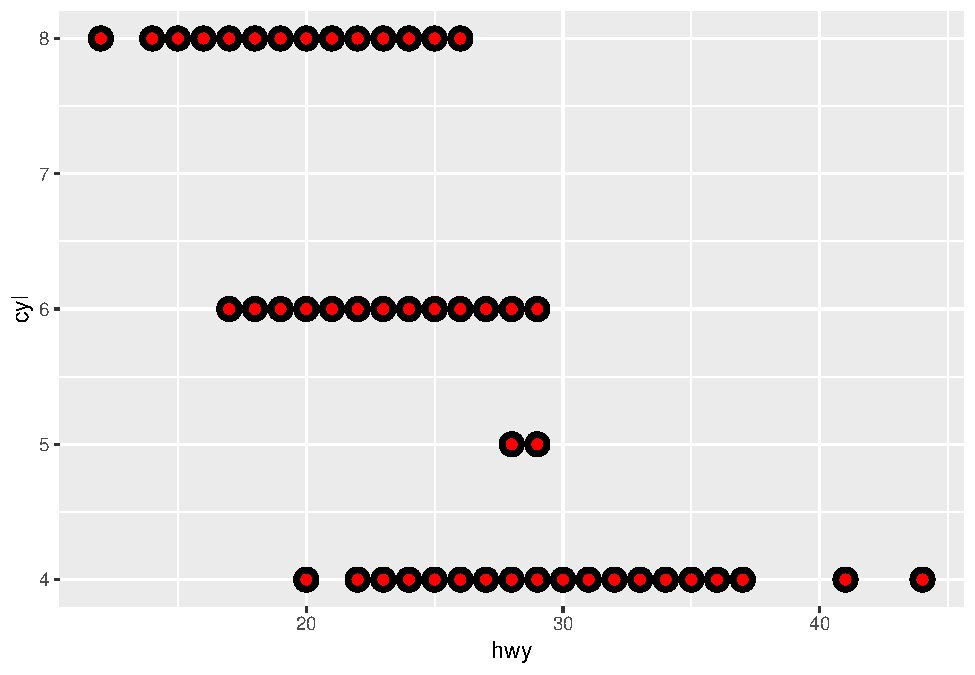
\includegraphics{homework_files/figure-latex/unnamed-chunk-16-1.pdf}

Ну а теперь \(5\)

\begin{Shaded}
\begin{Highlighting}[]
\KeywordTok{ggplot}\NormalTok{(mpg, }\KeywordTok{aes}\NormalTok{(hwy, cyl)) }\OperatorTok{+}
\StringTok{ }\KeywordTok{geom_point}\NormalTok{(}\DataTypeTok{shape=}\DecValTok{21}\NormalTok{,}\DataTypeTok{colour=}\StringTok{"black"}\NormalTok{,}\DataTypeTok{fill=}\StringTok{"red"}\NormalTok{,}\DataTypeTok{size=}\DecValTok{3}\NormalTok{,}\DataTypeTok{stroke=}\DecValTok{5}\NormalTok{)}
\end{Highlighting}
\end{Shaded}

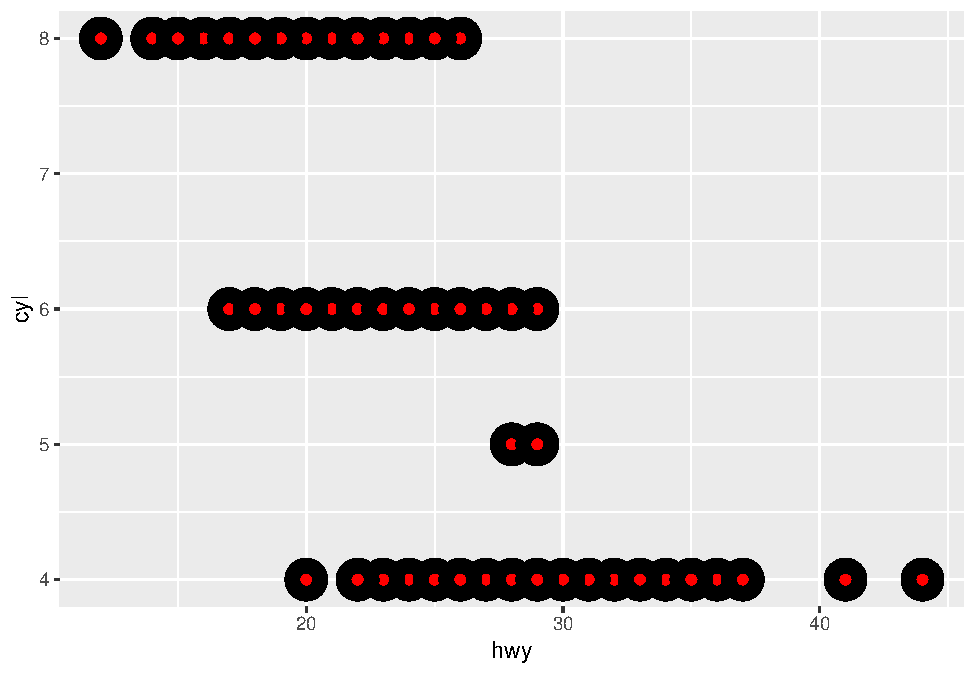
\includegraphics{homework_files/figure-latex/unnamed-chunk-17-1.pdf}

\subsection*{Упражнения 3.3.6}\label{-3.3.6}
\addcontentsline{toc}{subsection}{Упражнения 3.3.6}

What happens if you map an aesthetic to something other than a variable
name, like \texttt{aes(colour\ =\ displ\ \textless{}\ 5)}?

Визуальные атрибуты можно задавать и логическими выражениями, как
допустим в таком выражении:

\begin{Shaded}
\begin{Highlighting}[]
 \KeywordTok{ggplot}\NormalTok{(mpg, }\KeywordTok{aes}\NormalTok{(displ,hwy, }\DataTypeTok{color =}\NormalTok{ displ }\OperatorTok{<}\StringTok{ }\DecValTok{2}\NormalTok{)) }\OperatorTok{+}
\StringTok{   }\KeywordTok{geom_point}\NormalTok{()}
\end{Highlighting}
\end{Shaded}

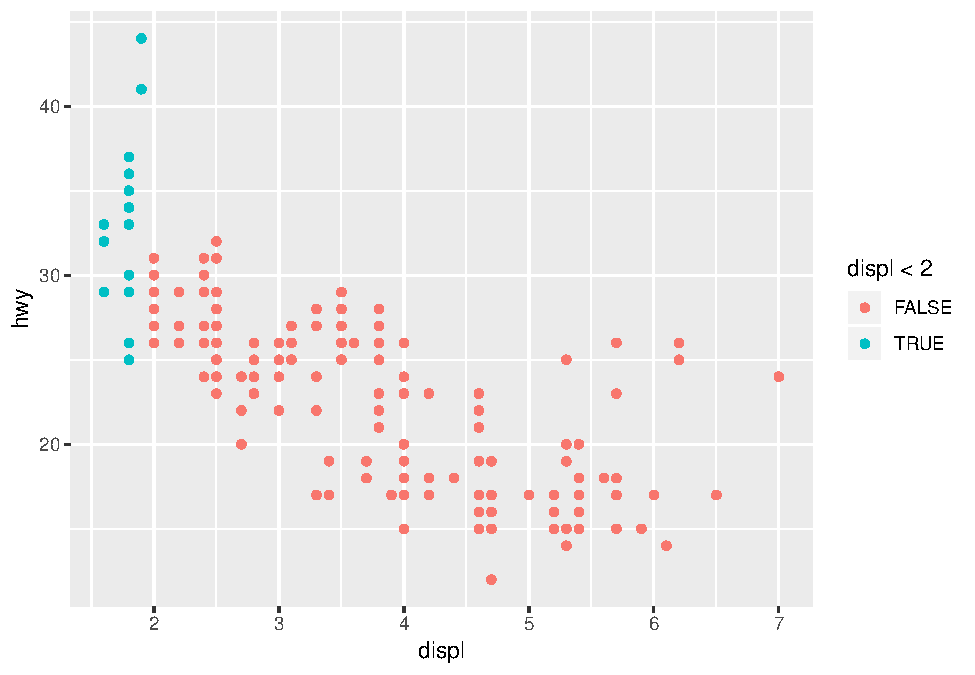
\includegraphics{homework_files/figure-latex/unnamed-chunk-18-1.pdf}

\begin{Shaded}
\begin{Highlighting}[]
 \KeywordTok{ggplot}\NormalTok{(mpg, }\KeywordTok{aes}\NormalTok{(displ,hwy, }\DataTypeTok{color =}\NormalTok{ displ }\OperatorTok{<}\StringTok{ }\DecValTok{4}\NormalTok{)) }\OperatorTok{+}
\StringTok{   }\KeywordTok{geom_point}\NormalTok{()}
\end{Highlighting}
\end{Shaded}

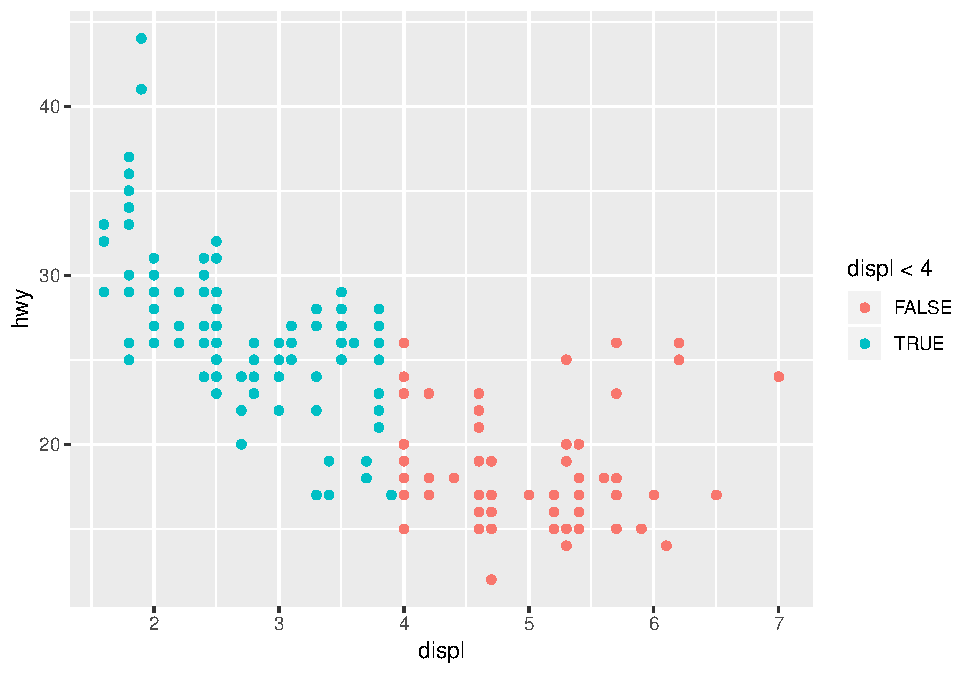
\includegraphics{homework_files/figure-latex/unnamed-chunk-19-1.pdf}

\begin{Shaded}
\begin{Highlighting}[]
 \KeywordTok{ggplot}\NormalTok{(mpg, }\KeywordTok{aes}\NormalTok{(displ,hwy, }\DataTypeTok{size =}\NormalTok{ displ }\OperatorTok{>}\StringTok{ }\DecValTok{3}\NormalTok{)) }\OperatorTok{+}
\StringTok{   }\KeywordTok{geom_point}\NormalTok{()}
\end{Highlighting}
\end{Shaded}

\begin{verbatim}
## Warning: Using size for a discrete variable is not advised.
\end{verbatim}

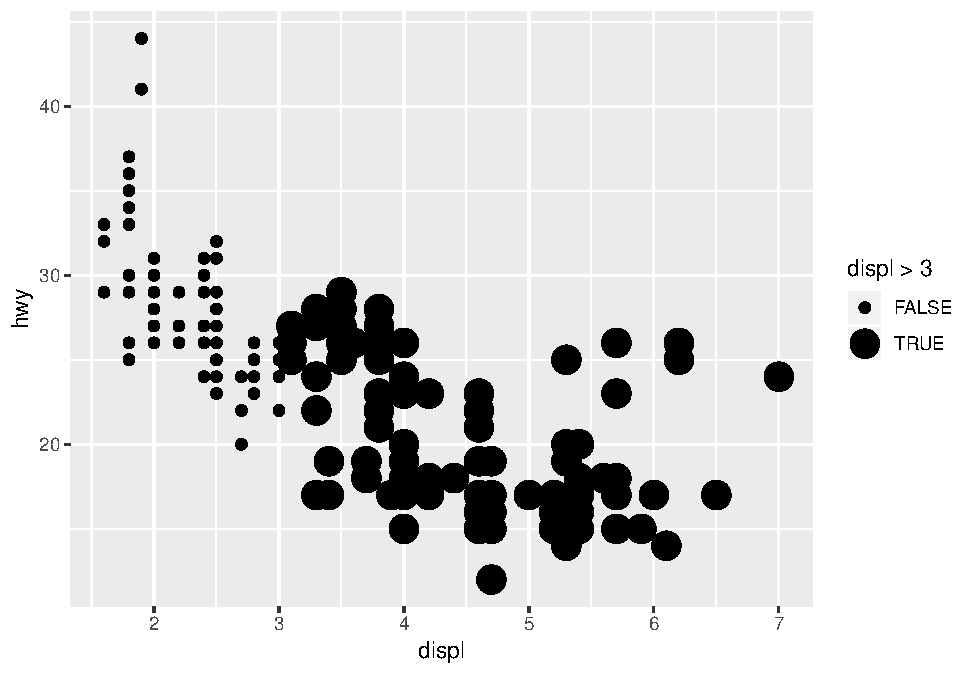
\includegraphics{homework_files/figure-latex/unnamed-chunk-20-1.pdf}

К тому же \texttt{R} ругается, что лучше бы такое не делать \#\#
Распространённые ошибки Проблемы случаются и это норм. Если что-то не
получается, чекни код.

Часто бывает что поставил \texttt{+} не туда. Он должен быть в конце
строки, а не в начале.

\section{Панели}

\subsection*{Упражнение 3.5.1}\label{-3.5.1}
\addcontentsline{toc}{subsection}{Упражнение 3.5.1}

What happens if you facet on a continuous variable? Как это работает.

Построим график \texttt{highway\ miles\ per\ gallon} от
\texttt{engine\ displacement,\ in\ litres}.

\begin{Shaded}
\begin{Highlighting}[]
\KeywordTok{ggplot}\NormalTok{(mpg, }\KeywordTok{aes}\NormalTok{(}\DataTypeTok{x =}\NormalTok{ displ, }\DataTypeTok{y =}\NormalTok{ hwy)) }\OperatorTok{+}
\StringTok{   }\KeywordTok{geom_point}\NormalTok{()}
\end{Highlighting}
\end{Shaded}

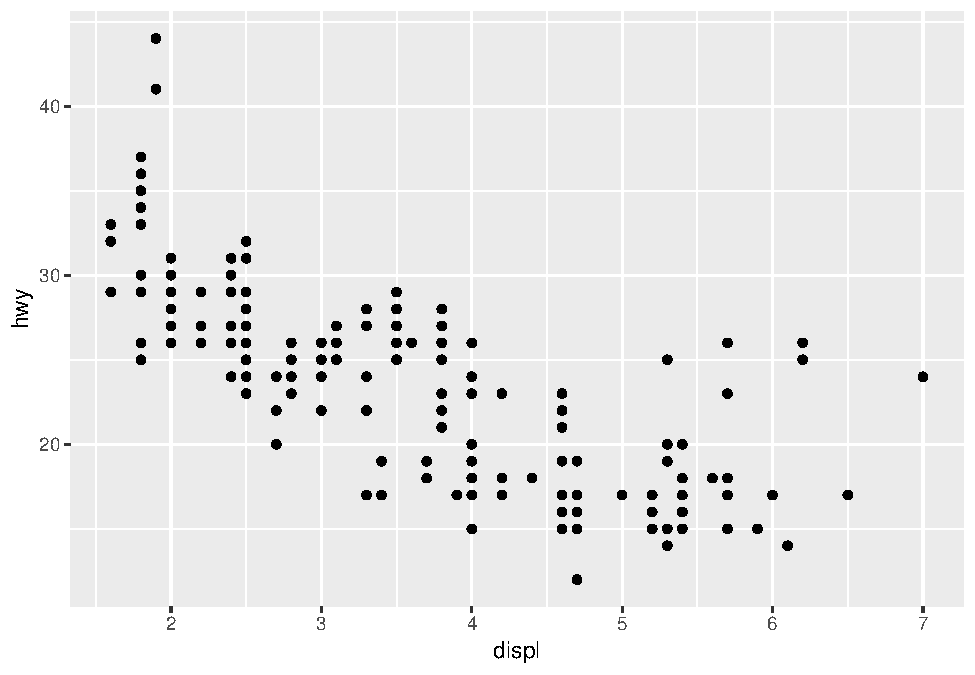
\includegraphics{homework_files/figure-latex/unnamed-chunk-21-1.pdf}

Теперь разделим на ``окошки'' т.е. возьмём срез графиков с теми же
дискретными переменными, но в разрезе типа привода автомобиля
\texttt{drv} от количества цилиндров \texttt{cyl}.

\begin{Shaded}
\begin{Highlighting}[]
\KeywordTok{ggplot}\NormalTok{(mpg, }\KeywordTok{aes}\NormalTok{(}\DataTypeTok{x =}\NormalTok{ displ, }\DataTypeTok{y =}\NormalTok{ hwy)) }\OperatorTok{+}
\StringTok{  }\KeywordTok{geom_point}\NormalTok{() }\OperatorTok{+}
\StringTok{  }\KeywordTok{facet_grid}\NormalTok{(drv}\OperatorTok{~}\StringTok{ }\NormalTok{cyl)}
\end{Highlighting}
\end{Shaded}

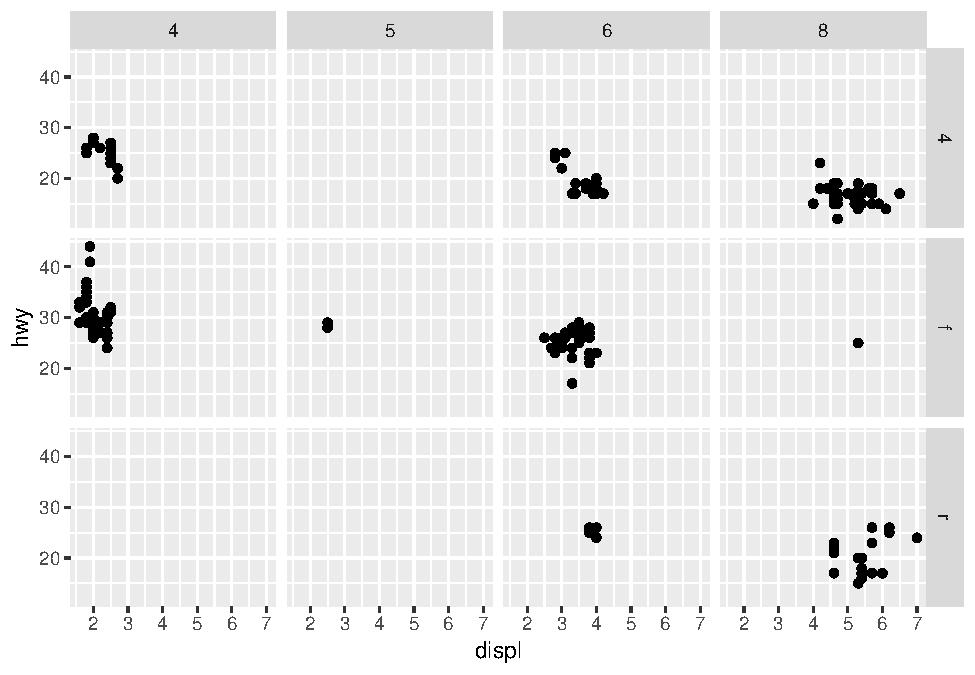
\includegraphics{homework_files/figure-latex/unnamed-chunk-22-1.pdf}
Получилось \(12\) панелей, потому что \texttt{drv} дискретная,
ограниченная переменная, у неё всего три набора значения (\(4, f, d\)).
Количество цилиндров \texttt{cyl} тоже ограниченная \(4,5,6,8\). Поэтому
получилось \(3*4=12\) значений. Так как панелей получилось немного,
такое представление осязаемо, с ним можно работать, оно информативно.

Если мы попробуем построить в одном измерении непрерывную переменную. То
количество панелей возрастёт на количество значений этой переменной.
Получится не очень информативно. Заменим в этом же построении количество
цилиндров \texttt{cyl} на расстояние, пройденное за один галлон топлива
в городской черте \texttt{cty}. Это непрерывная переменная, у которой
много значений.

\begin{Shaded}
\begin{Highlighting}[]
\KeywordTok{ggplot}\NormalTok{(mpg, }\KeywordTok{aes}\NormalTok{(}\DataTypeTok{x =}\NormalTok{ displ, }\DataTypeTok{y =}\NormalTok{ hwy)) }\OperatorTok{+}
\StringTok{ }\KeywordTok{geom_point}\NormalTok{() }\OperatorTok{+}
\StringTok{ }\KeywordTok{facet_grid}\NormalTok{(drv}\OperatorTok{~}\NormalTok{cty)}
\end{Highlighting}
\end{Shaded}

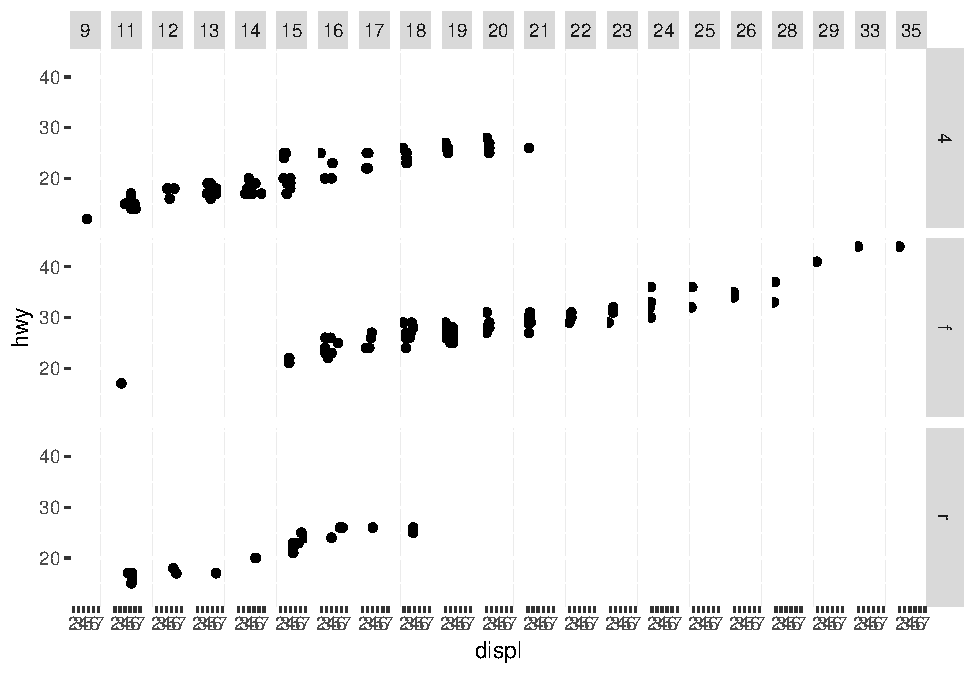
\includegraphics{homework_files/figure-latex/unnamed-chunk-23-1.pdf} Вот
что произойдет, если параметром для панели задать непрерывную
переменную. Будет много окошек, информативность представленной
информации падает.

\subsection*{Упражнение 3.5.2}\label{-3.5.2}
\addcontentsline{toc}{subsection}{Упражнение 3.5.2}

What do the empty cells in plot with
\texttt{facet\_grid(drv\ \textasciitilde{}\ cyl)} mean? How do they
relate to this plot?

Построим панели по заданному условию

\begin{Shaded}
\begin{Highlighting}[]
\KeywordTok{ggplot}\NormalTok{(mpg, }\KeywordTok{aes}\NormalTok{(}\DataTypeTok{x =}\NormalTok{ displ, }\DataTypeTok{y =}\NormalTok{ hwy)) }\OperatorTok{+}
\StringTok{    }\KeywordTok{geom_point}\NormalTok{() }\OperatorTok{+}
\StringTok{    }\KeywordTok{facet_grid}\NormalTok{(drv}\OperatorTok{~}\NormalTok{cyl)}
\end{Highlighting}
\end{Shaded}

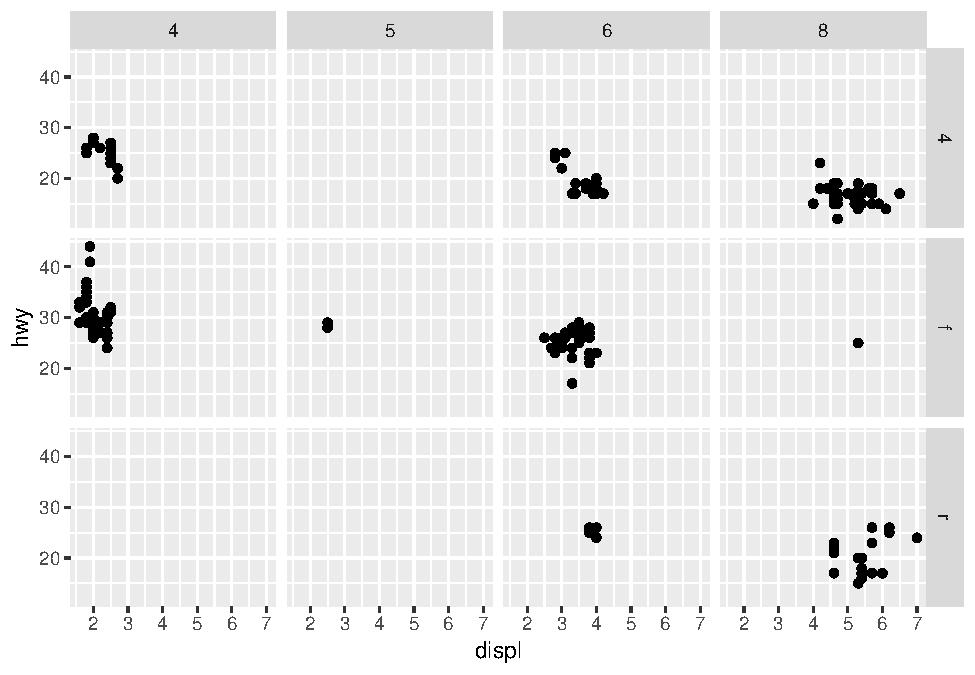
\includegraphics{homework_files/figure-latex/unnamed-chunk-24-1.pdf}

Пустые ячейки

\begin{itemize}
\tightlist
\item
  \(cyl(5):drv(4)\);
\item
  \(cyl(4):drv(r)\);
\item
  \(cyl(5):drv(r)\);
\end{itemize}

говорят о том, что нет точек удовлетворяющих этим разрезам данных. Иначе
говоря, в наборе данных \texttt{mpg}

\begin{itemize}
\tightlist
\item
  нет полноприводных авто с 5 цилиндрами
\item
  заднеприводных авто с 4 цилиндрами
\item
  заднеприводных авто с 5 цилиндрами
\end{itemize}

Построение функции

\begin{Shaded}
\begin{Highlighting}[]
\KeywordTok{ggplot}\NormalTok{(}\DataTypeTok{data =}\NormalTok{ mpg) }\OperatorTok{+}\StringTok{ }
\StringTok{  }\KeywordTok{geom_point}\NormalTok{(}\DataTypeTok{mapping =} \KeywordTok{aes}\NormalTok{(}\DataTypeTok{x =}\NormalTok{ drv, }\DataTypeTok{y =}\NormalTok{ cyl))}
\end{Highlighting}
\end{Shaded}

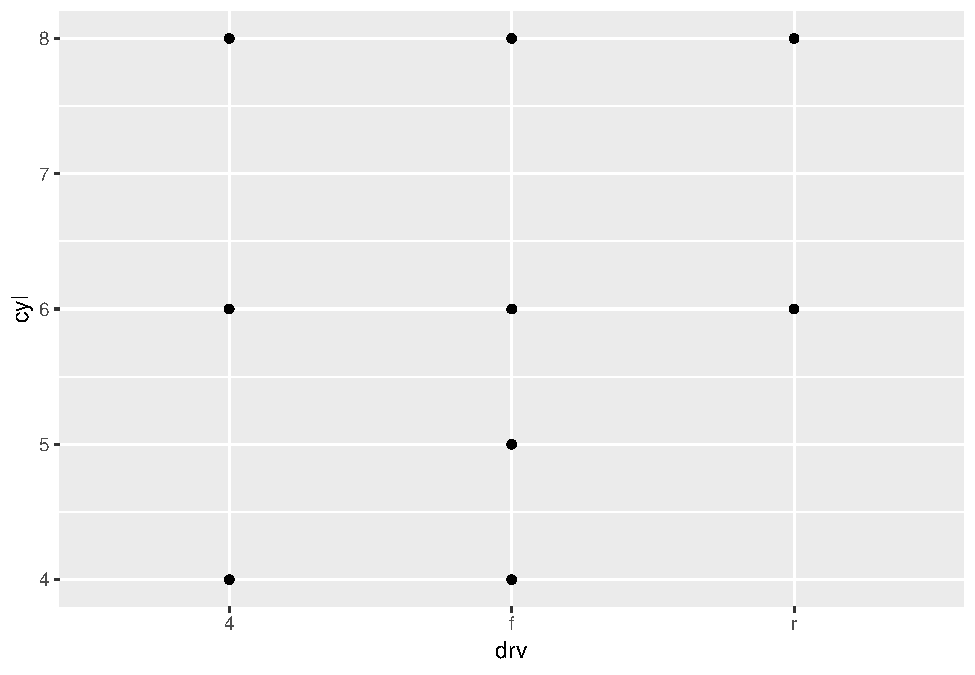
\includegraphics{homework_files/figure-latex/unnamed-chunk-25-1.pdf}

\subsection*{Упражнение 3.5.3}\label{-3.5.3}
\addcontentsline{toc}{subsection}{Упражнение 3.5.3}

What plots does the following code make? What does \texttt{«.»} do?

\begin{Shaded}
\begin{Highlighting}[]
\KeywordTok{ggplot}\NormalTok{(}\DataTypeTok{data =}\NormalTok{ mpg) }\OperatorTok{+}\StringTok{ }
\StringTok{  }\KeywordTok{geom_point}\NormalTok{(}\DataTypeTok{mapping =} \KeywordTok{aes}\NormalTok{(}\DataTypeTok{x =}\NormalTok{ displ, }\DataTypeTok{y =}\NormalTok{ hwy)) }\OperatorTok{+}
\StringTok{  }\KeywordTok{facet_grid}\NormalTok{(drv }\OperatorTok{~}\StringTok{ }\NormalTok{.)}
\end{Highlighting}
\end{Shaded}

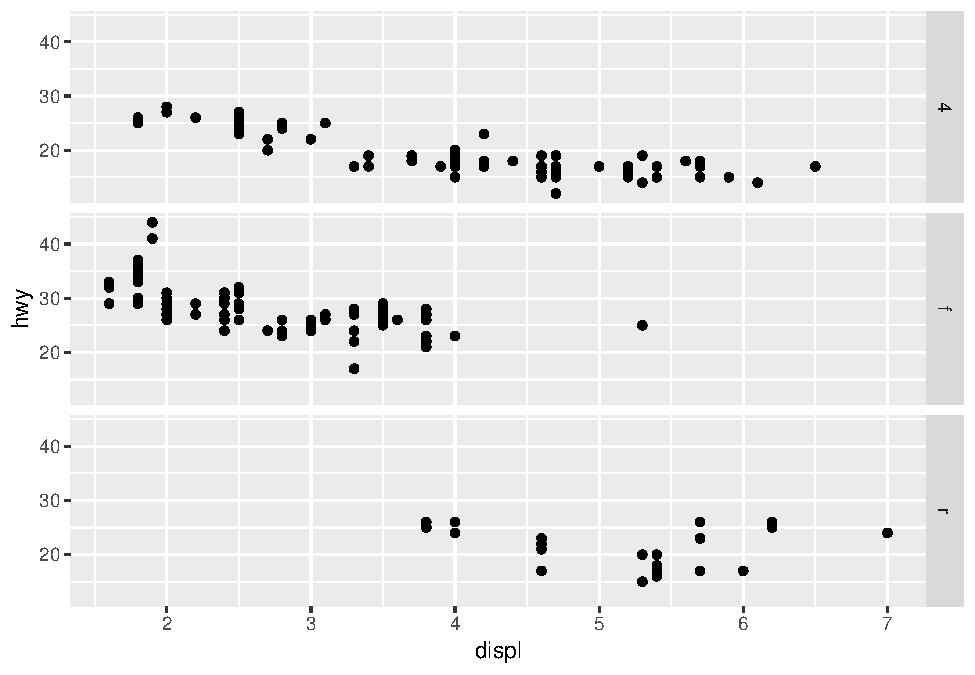
\includegraphics{homework_files/figure-latex/unnamed-chunk-26-1.pdf}

ggplot(data = mpg) + geom\_point(mapping = aes(x = displ, y = hwy)) +
facet\_grid(. \textasciitilde{} cyl)

\bibliography{book.bib,packages.bib}


\end{document}
